\documentclass[9pt]{sigplanconf}

\usepackage{amssymb}
\usepackage{amsmath}
\usepackage{amsthm}
\usepackage{stmaryrd}
\usepackage{color}
\usepackage{graphics}
\usepackage{fancyvrb}
\usepackage{subfigure}
\usepackage{amsthm}
\usepackage{tikz}

\CustomVerbatimEnvironment{SpecVerbatim}{Verbatim}{fontsize=\footnotesize,xleftmargin=0.65cm,
xrightmargin=0.2cm,commandchars=\\\{\},baselinestretch=0.97}
\CustomVerbatimEnvironment{ExmVerbatim}{Verbatim}{fontsize=\footnotesize,xleftmargin=0.65cm,
xrightmargin=0.2cm,baselinestretch=0.97,numbers=left}
\CustomVerbatimEnvironment{IVerbatim}{Verbatim}{fontsize=\relsize{-1},xleftmargin=0.65cm,
xrightmargin=0.2cm,commandchars=\\\{\},baselinestretch=0.97}


\definecolor{darkgreen}{rgb}{0.0,0.5,0.0}
\definecolor{darkpurple}{rgb}{0.6,0.0,0.6}
\definecolor{orange}{rgb}{0.8,0.4,0.0}
\definecolor{darkorange}{rgb}{0.5,0.2,0.0}
\definecolor{marco}{rgb}{0.0,0.3,0.5}
\definecolor{gray}{rgb}{0.2,0.2,0.2}

\newcommand{\bn}{\mathbb{N}}

\newcommand{\dnote}[1]{\textcolor{darkpurple}{Dom: #1}}
\newcommand{\mnote}[1]{\textcolor{darkgreen}{Mistral: #1}}

\newcounter{block}

\newtheorem{lemma}[block]{Lemma}
\newtheorem{proposition}[block]{Proposition}
%\newtheorem{definition}[block]{Definisssstion}

\theoremstyle{definition}

\newtheorem{theorem}[block]{Theorem}
\newtheorem{remark}[block]{Remark}
\newtheorem{example}[block]{Example}
\newtheorem{definition}[block]{Definition}

% Writing macros
\newcommand{\ie}{\emph{i.e..}}
\newcommand{\eg}{\emph{e.g.}}

\newcommand{\dimId}{\texttt{dim}}

% Semantics related
\newcommand{\interp}[1]{\llbracket{#1}\rrbracket}

% Syntax macros
\newcommand{\nonterm}[1]{\textit{#1}}
\newcommand{\term}[1]{\texttt{#1}}

\newcommand{\stenFwd}[2]{\texttt{forward} \, (\texttt{depth=}#1,
  \texttt{dim=}#2)}
\newcommand{\stenBwd}[2]{\texttt{backward} \, (\texttt{depth=}#1,
  \texttt{dim=}#2)}
\newcommand{\stenCen}[2]{\texttt{centered} \, (\texttt{depth=}#1,
  \texttt{dim=}#2)}

\title{Time and space specifications for stencils}
\authorinfo{}{}

\begin{document}
\maketitle

\begin{abstract}
\end{abstract}

\bibliographystyle{plain}

\section{Introduction}

\emph{Stencils} are a ubiquitous programming pattern, common in
scientific and numerical computing applications. Informally, a stencil
computation computes an array value, where the value at each index $i$ of
this array is calculated from a \emph{neighbourhood} of values around $i$ in
some input array(s), \eg{}, the Game of Life, convolutions in image
processing, approximations to differential equations. For example, the
following iteratively computes the one-dimensional discrete Laplace
transform (an approximation to a derivative): 
%
\begin{ExmVerbatim}
do iter = 0, itermax
   do i = 1, (n-1)
      b(i) = a(i-1) - 2*a(i) + a(i+1)
   a = b
\end{ExmVerbatim}
%
Line 3 is the core of the stencil computation, calculating
the value at \texttt{b(i)} from a neighbourhood of elements about
\texttt{a(i)}. Line 4 swaps
\texttt{a} and \texttt{b} between iterations, where \texttt{b} becomes the
input for the next iteration. (Note, we use the parentheses syntax
\texttt{( )} for
array subscripts rather than the bracket syntax \texttt{[ ]}. 

%This stencil computation exhibits statically decideable
%spatial and temporal relationships between $\texttt{a}$ and
%$\texttt{b}$.
In this simple example, the dependencies between between \texttt{a}
and \texttt{b} form a simple spatial relationship which is easily
understood. This spatial relationship determines other aspects of the
program and its efficient implementation: how much ``boundary'' is
needed for the array, the most cache-efficient layout in memory,
the partitioning shape for parallel implementations. 

More complex stencil computations can be much harder to understand and
subsequently more prone to error. For example,
Figure~\ref{ref:navier-stokes-fragment} shows three lines from a
Navier-Stokes fluid simulator in which two arrays are read from with
different data access patterns, across two dimensions. The interaction
is much harder to understand, with the potential for the developer to
accidentally introduce an error via simple textual mistakes, for
example writing $\texttt{(i-1,j)}$ instead of $\texttt{(i+1,j)}$.

In this work, we introduce a simple specification language for the
spatial and temporal properties of stencil comptuations. The
specifications abstract over the fine grained detail of stencil access
patterns.  In practise, most stencil computations have a regular shape
that can be described simply and abstractly, with a small set of
coarse-grained descriptions. In the case of our first Laplace example,
our inference procedure provides the specification:
%
\begin{SpecVerbatim}
!=  stencil centered (depth=1, dim=1) :: a
!=  stencil dependency a, mutual       :: b
\end{SpecVerbatim}
%
The first line explains that \texttt{a} is read from with a
symmetrical stencil pattern (``centered'') to a depth of one in each
direction in its first (and only) dimension.  The second line explains
the temporal relationship between \texttt{b} and \texttt{a}: that
previous time step for \texttt{b} is actually provided by \texttt{a},
and vice versa. This is explained as a mutual dependence between
\texttt{a} and \texttt{b}. In the case of the Navier-Stokes example of
Figure~\ref{ref:navier-stokes-fragment}, its inferred specification is shown
in Figure~\ref{ref:navier-stokes-fragment}(b). The 
specification explains that, over the whole fragment, \texttt{u} is
read from with a centered pattern to depth of 1 in both dimensions
(this is known as the \emph{five point stencil}) and \texttt{v}
is read from in a neighbourhood bounded by forward to depth of $1$ in
the first dimension and backward to a depth of $1$ in the second
dimension. These can drawn pictorially as follows where the horizontal
dimensions is \text{dim=1} and the vertical is \texttt{dim=2}:

\begin{center}
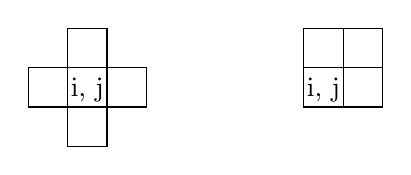
\begin{tikzpicture}
\node at (1.25,1.22) {i, j};
\draw (1,1) rectangle (1.5,1.5);
\draw (1.5,1) rectangle (2,1.5);
\draw (1,0.5) rectangle (1.5,1);
\draw (0.5,1) rectangle (1,1.5);
\draw (1,1.5) rectangle (1.5,2);
%
\node at (4.25,1.22) {i, j};
\draw (4,1) rectangle (4.5,1.5);
\draw (4.5,1) rectangle (5,1.5);
\draw (4.5,1.5) rectangle (5,2);
\draw (4,1.5) rectangle (4.5,2);
\end{tikzpicture}
\end{center}


In this paper, we make the following contributions:
%
\begin{itemize}
\item we introduce a specification language for
stencil computations that captures many common forms
of data access pattern, both spatial and temporal (Section~\ref{sec:lang});
\item we detail inference and checking
algorithms for stencil specifications (Section~\ref{sec:analysis});
\item we evaluate our implementation of the approach
in the CamFort tool for Fortran verification, studying
a number of example programs to assess the usefulness
of this approach.
\dnote{insert results here}
\end{itemize}
%

\begin{figure}
\begin{ExmVerbatim}[firstnumber=20]
du2dx = ((u(i,j)+u(i+1,j))*(u(i,j)+u(i+1,j))+
    gamma*abs(u(i,j)+u(i+1,j))*(u(i,j)-u(i+1,j))-
    (u(i-1,j)+u(i,j))*(u(i-1,j)+u(i,j))-
    gamma*abs(u(i-1,j)+u(i,j))*(u(i-1,j)-u(i,j)))
    /(4.0*delx)

duvdy = ((v(i,j)+v(i+1,j))*(u(i,j)+u(i,j+1))+
   gamma*abs(v(i,j)+v(i+1,j))*(u(i,j)-u(i,j+1))-
   (v(i,j-1)+v(i+1,j-1))*(u(i,j-1)+u(i,j))-
   gamma*abs(v(i,j-1)+v(i+1,j-1))*(u(i,j-1)-u(i,j)))
   /(4.0*dely)

laplu = (u(i+1,j)-2.0*u(i,j)+u(i-1,j))/delx/delx+
          (u(i,j+1)-2.0*u(i,j)+u(i,j-1))/dely/dely
\end{ExmVerbatim}
(a). Excerpt from the Fortran code,
showing highly-detailed stencil computations. \\

%\begin{SpecVerbatim}[xleftmargin=0.1cm]
%20-24  u: centered depth=1 dim=1
%6-30  u: centered depth=1 dim=2
%      v: forward depth=1 dim=1, backward depth=1 dim=1
%32-33  u: centered depth=1 dim=1,2
%\end{SpecVerbatim}

\begin{SpecVerbatim}[xleftmargin=0.3cm]
!=   stencil centered(depth=1, dim=1)
           + centered(depth=1, dim=2) :: u

!=   stencil forward(depth=1, dim=1)
           * backward(depth=1, dim=2) :: v
\end{SpecVerbatim}
(b). Inferred stencil specification from CamFort
\caption{Fragment of Navier-Stokes fluid simulator and its specification}
\label{ref:navier-stokes-fragment}
\end{figure}

\section{Stencil specification language}
\label{sec:lang}

Our specification system is based on the observation
that most forms of array access in numberical code have
a fixed, statically-determined access pattern. For example, the
``\emph{five-point stencil}'' on a two-dimensional array reads from array
indices $(i, j)$, $(i-1, j)$, $(i+1, j)$, $(i, j-1)$, and $(i, j+1)$
for all $i, j$ within the inner boundary of the array (to avoid
out-of-bounds access at the edges). We revisit this hypothesis
in Section~\ref{sec:evaluation} where the inference of
such regular stencil patterns on a corpus of numerical programs (both
small and large). We found that indeed \dnote{..}.

We outline the specification language here. Section~\ref{sec:syntax}
oultines the syntax. Section~\ref{sec:semantics} defines its semantics
via a simple multi-set interpretation over indices. Section~\ref{sec:eqs} provides an
equational theory for specifications via relation ($\equiv$) and a
theory of approximation via relation ($<:$). These equations are then
proven sound with respecto the multi-set semantics of Section~\ref{sec:semantics}.

\subsection{Syntax}
\label{sec:syntax}

Figure~\ref{fig:syntax}
gives the syntax, which we introduces in stages below.
The top-level is given by the \textit{spec} production
which splits into either a \textit{spatial} specification or
a \textit{temporal specification}.
%%

\begin{figure}[t]
\begin{align*}
\def\arraystretch{1.2}
\setlength{\arraycolsep}{0.2em}
\newcommand{\dimTy}{\mathbb{D}}
\begin{array}{rl}
\nonterm{specification} ::= & \nonterm{regionDec} \mid \nonterm{specDec} \\
\nonterm{specDec} ::= & \term{stencil} \; \nonterm{spec}
  \\
\nonterm{regionDec} ::= &  \texttt{region} \; \nonterm{rvar} \; \texttt{=} \;
                         \nonterm{region}\\
\nonterm{spec} ::= & \nonterm{spatial} \mid \nonterm{temporal}   \\[1em]
\nonterm{spatial} ::= & [\nonterm{mod}] \;
                       [\nonterm{approxMod},] \; [\nonterm{region}] \\
\nonterm{mod} ::= & [\nonterm{modR},] \; [\nonterm{modRefl},] \; [\nonterm{modIrefl},] \\
\nonterm{modR} ::= &
 \term{readOnce} \\
\nonterm{modRefl} ::= & \term{reflexive}, \; \term{dims=}\dimTy \{\term{,} \; \dimTy\} \\
\nonterm{modIrrefl} ::= & \term{irreflexive}, \; \term{dims=}\dimTy \{\term{,}
          \dimTy\}\\
\nonterm{approxMod} ::= & \term{atMost} \; \mid \; \term{atLeast} \\[0.1em]
\nonterm{region} ::= & \term{forward}, \term{depth=}\mathbb{N}, \term{dim=}\dimTy  \\
\mid \; & \term{backward}, \term{depth=}\mathbb{N}, \term{dim=}\dimTy \\
\mid \; & \term{centered}, \term{depth=}\mathbb{N}, \term{dim=}\dimTy \\
\mid \; & \nonterm{region} \; \term{+} \; \nonterm{region} \\
\mid \; & \nonterm{region} \; \term{*} \; \nonterm{region} \\
\mid \; & \nonterm{rvar}  \\[0.5em]
\nonterm{temporal} ::= \; & \term{dependency} \; (v \; \{ , v \})
  \\[0.5em]
\dimTy ::= \; & \mathbb{N}_{>0} \\
\nonterm{rvar} ::= \; & [\text{\term{a}-\term{z}$\,$\term{A}-\term{Z}$\,$\term{0}-\term{9}}]+
\end{array}
\end{align*}
\caption{Specification syntax (EBNF grammar)}
\label{fig:syntax}
\end{figure}

\paragraph{Spatial specifications}


\paragraph{Temporal specifications}


\subsection{A semantic model for specifications}
\label{sec:semantics}

\newcommand{\relix}{(\mathbb{Z}_\bot)^\mathbb{D}}

We give a model of our specifications which explains
the range of indices which correspond to the specifications.
The model is based on multi-sets since array indices my be repeated
in an expression.

Figure~\ref{fig:model} describes the model in terms of
an interpretation function $\interp{-}$ which maps specifications
to multisets of relative indices.

\begin{definition}Relative indices are drawn
from $(\mathbb{Z}_{\bot})^{\mathbb{D}}$, essentially an infinite
tuple of offsets. For example, $(i, j+1)$ corresponds to
the relative index $(0, 1, \bot, \bot, \ldots)$
\end{definition}

The main interpretation function is overloaded on lists of
variable-spec pairs $\interp{\overline{v : S}}$,
returning multisets of variable-relative-index pairs. This provides
the top-level definition of the model, with $\interp{-}$ overloaded
on $S$, $\interp{S}$ mqpping to multisets of
relative indices not associated to an array avariable.

\begin{figure}
\newcommand{\singleEntry}[2]{\textbf{J}_{#2}^{#1}}
\begin{align*}
%
% REGION model
%
\interp{\stenFwd{k}{d}}^r_n & =
 \{i\singleEntry{d}{n} \mid i \in \{0, \ldots, k\} \} \\
\interp{\stenBwd{k}{d}}^r_n & =
 \{i\singleEntry{d}{n} \mid i \in \{-k, \ldots, 0\} \} \\
\interp{\stenCen{k}{d}}^r_n & =
 \{i\singleEntry{d}{n} \mid i \in \{-k, \ldots, k\} \} \\
%
% REGION PROD model
%
\interp{r_1 \; \texttt{$\ast$} \, \ldots \, \texttt{$\ast$} \; r_m}^{\ast}_n &
= \interp{r_1}^r_n \otimes \ldots \otimes \interp{r_m}^r_n \\
%
%  REGION SUM model
%
\interp{r_1 \; \texttt{+} \, \ldots \, \texttt{+} \; r_m}^{+}_n &
= \interp{r_1}^{\ast}_n \cup \ldots \cup \interp{r_m}^{\ast}_n \\
\end{align*}
%where $\singleEntry
TODO: insert explanation for the $\textbf{J}$ notation (see Matrix
textbook).


%\textit{$a^m \in A$ means there are $n$ copies of $a$ in
%  the multi-set $A$}
\caption{Multi-set model of specifications}
\label{fig:model}
\end{figure}

\subsection{Equational theory and approximations}
\label{sec:eqs}

Figure~\ref{fig:equations}

\begin{figure}
\begin{align*}
\hspace{-1em}
\setlength{\arraycolsep}{0.05em}
\begin{array}{c}
\framebox{$\overline{\texttt{v} : S} \equiv \overline{\texttt{u} : T}$} \\[1em]
\begin{array}{rl}
(\textsc{coalesceF}) \;\; & (\texttt{a} : \texttt{fwd} \;
                       \texttt{dims}=ds \; \texttt{depth}=n; \\
&  \;\, \texttt{a} :  \texttt{fwd} \; \texttt{dims}=ds \; \texttt{depth}=n+1)\\
\equiv \; & \texttt{a} :  \texttt{fwd} \; \texttt{depth}=n+1,
         \texttt{dims}=ds \\[0.75em]
(\textsc{coalesceB}) \;\; & (\texttt{a} : \texttt{bwd} \;
                       \texttt{dims}=ds \; \texttt{depth}=n; \\
&  \;\, \texttt{a} :  \texttt{bwd} \; \texttt{dims}=ds \; \texttt{depth}=n+1) \\
\equiv \; & \texttt{a} :  \texttt{bwd} \; \texttt{depth}=n+1,
         \texttt{dims}=ds \\[0.75em]
(\textsc{idem}) \;\; & (\texttt{a} : S; \texttt{a} : S) \equiv (\texttt{a}
                  : S)
\end{array} \\ \\
\framebox{$\texttt{v} : S \equiv \texttt{v'} : S'$} \\[1em]
\begin{array}{ll}
(\texttt{a} : \; \texttt{bwd} \; \texttt{depth=1\{b\}} \;
  \texttt{dim=t})
\, & \equiv \,
(\texttt{b} : \; \texttt{bwd} \; \texttt{depth=1\{a\}} \;
  \texttt{dim=t})
\\
(\texttt{a} : \; \texttt{fwd} \; \texttt{depth=1\{b\}}\;
  \texttt{dim=t})
\, & \equiv \,
(\texttt{b} : \; \texttt{fwd} \; \texttt{depth=1\{a\}} \;
  \texttt{dim=t})
\end{array}
\\ \\
\framebox{$S \equiv S'$} \\[0.75em]
\begin{array}{ll}
(a : \texttt{read-once} \; S) \; & \equiv \; (a : \texttt{read-once} \;\,
  \texttt{read-once} \; \, S)
\end{array}
\end{array}
\end{align*}
\caption{Equations on specifications}
\label{fig:equations}
\end{figure}


\begin{theorem}[Soundness]
\[
\overline{\texttt{v} : S}\equiv \overline{\texttt{u} : T}
\; \Rightarrow \;
\interp{\overline{\texttt{v} : S}} = \interp{\overline{\texttt{u} : T}}
\]
\end{theorem}

\paragraph{Proof} (see Appendix)


\subsubsection{Safety and sub-specifications}

Figure~\ref{fig:inequations}

\begin{figure}[t]
{\framebox{
\begin{minipage}{0.88\linewidth}
\begin{align*}
\hspace{-0.7em}
\begin{array}{c}
\dfrac{}{S <: S}(\textsc{refl}) \qquad \dfrac{R <: S \quad S <: T}{R <:
  T}(\textsc{trans}) \\[1.5em]
\dfrac{}{S <: \; \texttt{unspecified dims=}ds}(\top)
\\[1.5em]
\dfrac{}{\texttt{read-once} \, S <: S}(\textsc{rep})
\\[1.5em]
\setlength{\arraycolsep}{0.1em}
\dfrac{\hspace{3em} ds \subseteq es \; \wedge \; n \leq m \hspace{3em}}
{\begin{array}{rl}
\texttt{fwd} \; \texttt{depth=}n \; \texttt{dim=}ds & <: \texttt{fwd} \;
  \texttt{depth=}m \; \texttt{dim=}es
%& \;\, ds \subseteq es \wedge n \leq m
\\
\wedge \; \texttt{bwd} \; \texttt{depth=}n \; \texttt{dim=}ds & <: \texttt{bwd} \;
  \texttt{depth=}m \; \texttt{dim=}es
%& \;\, ds \subseteq es \wedge n \leq m
\\
\wedge \; \texttt{fwd} \; \texttt{depth=}n \; \texttt{dim=}ds & <: \texttt{sym} \;
  \texttt{depth=}m \; \texttt{dim=}es
%& \;\, ds \subseteq es \wedge n \leq m
\\
\wedge \; \texttt{bwd} \; \texttt{depth=}n \; \texttt{dim=}ds & <: \texttt{sym} \;
  \texttt{depth=}m \; \texttt{dim=}es
\end{array}}
%{\footnotesize{(\textsc{cover})}}
%\hspace{-0.1em}
\end{array}
\end{align*}
\end{minipage}}}
\caption{Definition of sub-specification relation}
\label{fig:inequations}
\end{figure}


\begin{theorem}[Soundness]
\[
\overline{\texttt{v} : S} <: \overline{\texttt{u} : T}
\; \Rightarrow \;
\interp{\overline{\texttt{v} : S}} \subseteq \interp{\overline{\texttt{u} : T}}
\]
\end{theorem}

\paragraph{Proof} (see Appendix)



\section{Examples and common patterns}

% Implicit vs explicit differentiation methods
% (forward implicit needs 'solver')
% backward - Euler
% runge-kutta 2nd-order

\begin{example}[FTCS (Forward time, centered space)]

  Otherwise known as the \emph{explicit method}, is a common
  pattern since it tends to be more efficient than other approches
  (see BTCS and CTCS below). However, its disadvantage is that it is
  unstable if the resolution is not well chosen.

\begin{ExmVerbatim}
b(x) = a(x) + r*(a(x-1) - 2*a(x) + a(x+1))
\end{ExmVerbatim}
%
For this statement, the inference provides the specification:
%
\begin{SpecVerbatim}
!=  stencil centered, depth=1, dim=0 :: a
\end{SpecVerbatim}



\end{example}

\paragraph{BTCS (Backward time, centered space) -- implicit method}

\paragraph{CTCS (Centered time, centered space) - Crank-Nicolson method}

\section{Specification inference and checking}
\label{sec:analysis}

\mnote{Few cases that we might like to consider (there are examples
    of each in \#camfort-main Slack channel):
  \begin{itemize}
    \item Matrix operator overloading $a + b$, where both are arrays
    \item Scalar operator overloading $a + b$, where a is an array b is a
      scalar. $b$ is added to all.
    \item Sliding. $a = b$ where the dimensionsare $a(1:10)$, $b(2:11)$,
      so the assignment causes shifting.
  \end{itemize}
}

In the following, we defined
\emph{base induction variables} to be the variables
 defined by a ``for'' loop (\eg{}, that get incremented each time the
loop is re-entered).

\begin{definition}[Constant translations]
An indexing expression $e$ is a \emph{constant translation} if,
for a base induction variable $i$, then $e \equiv i + a$ or $e \equiv i - a$
where $a$ is a constant. The relation $\equiv$ identifies terms
up-to commutativity of $+$ and the inverse
relation of $+$ and $-$ (\eg{}, $(-b) + i \equiv i - b$).
In the following, we classify constant translation expressions
using the predicate $\textsf{trans}$.
\end{definition}

\paragraph{Step 1: Data-access analysis}

\dnote{Might want to do 'stencil' (gather) and 'mould' (scatter)
  patterns separately}
\begin{align*}
\begin{array}{lll}
\interp{e_1 = e_2}    & = \interp{e_2} \\
\interp{e_1 e_2}      & = \interp{e_1} \cup \interp{e_2} \\
\interp{a(\tilde{e})} & = \{e | e \in \tilde{e}, \textsf{trans}(e)\} & \textit{where each $e \in
                                          \tilde{e}$ is a constant or constant translation}
\end{array}
\end{align*}

Index analysis is a \emph{coeffect analysis}.

\paragraph{Step 2: Coalesce contiguous indices into regions}

% fairly mechanical

\subsection{Infering temporal specifications}

The reserved dimension \dimId{t}

\section{Evaluation}
\label{sec:evaluation}

\section{Discussion}
\label{sec:discussion}


\bibliography{references}


\onecolumn
\appendix

\section{Correctness}


\begin{theorem}[Soundness]
\[
\overline{\texttt{v} : S}\equiv \overline{\texttt{u} : T}
\; \Rightarrow \;
\interp{\overline{\texttt{v} : S}} = \interp{\overline{\texttt{u} : T}}
\]
\end{theorem}

\paragraph{Proof}
\begin{itemize}
\item \textsc{coalesceF}
\begin{align*}
\llbracket & \texttt{v} : \texttt{fwd} \; \texttt{dims}=ds \; \texttt{depth}=n; \,
  \texttt{v} :  \texttt{fwd} \; \texttt{dims}=ds \;
  \texttt{depth}=n+1)\rrbracket \\
& =  \{ (\texttt{v}, ix)^m \mid \forall \, m, ix : \relix, d : \mathbb{N}
  \, . \, d \in \textit{ds} \Rightarrow ix \, d \leq (n+1) \} \; \cup \; \{ ix^m \mid \forall \, m, ix : \mathbb{Z}^{\mathbb{N}}, d : \mathbb{N}
  \, . \, d \in \textit{ds} \Rightarrow ix \, d \leq n \}\\
& =  \{ (\texttt{v}, ix)^m \mid \forall \, m, ix : \relix, d : \mathbb{N}
  \, . \, d \in \textit{ds} \Rightarrow ((ix \, d \leq (n+1)) \vee (ix \,
  d \leq n)) \} \\
& =  \{ (\texttt{v}, ix)^m \mid \forall \, m, ix : \relix, d : \mathbb{N}
  \, . \, d \in \textit{ds} \Rightarrow ix \, d \leq (n+1) \} \\
& = \interp{\texttt{v} : \texttt{fwd} \; \texttt{dim}=ds \;
  \texttt{depth}=n + 1} \qquad \Box
\end{align*}
\end{itemize}

\end{document}
